\documentclass[tikz,margin=0pt]{standalone}

%\setlength{\paperwidth}{108mm}
%\setlength{\paperheight}{210mm}
%\ifx\pdfoutput\undefined
%\else
%\setlength{\pdfpagewidth}{\paperwidth}
%\setlength{\pdfpageheight}{\paperheight}
%\fi

%\usepackage{tikz}
\usepackage{comment}
\usetikzlibrary{positioning}

\pgfdeclarelayer{bg}    % declare background layer
\pgfsetlayers{bg,main}  % set the order of the layers (main is the standard layer)

\begin{document}
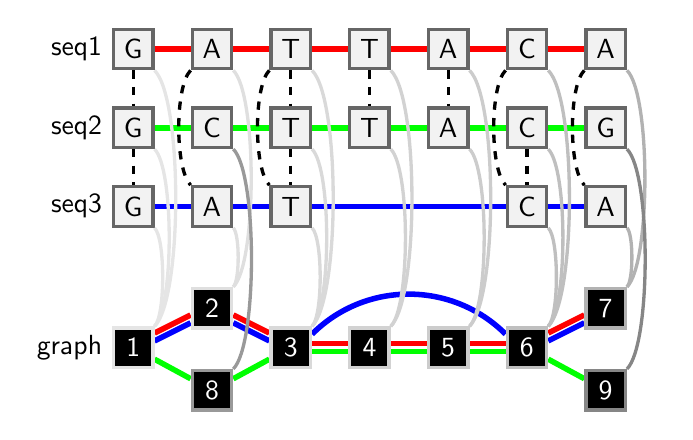
\begin{tikzpicture}[auto,
    node distance= 10mm and 20mm,
    font=\sffamily,
    roundnode/.style={circle, draw=black!60, fill=gray!10, very thick, minimum size=7mm},
    squarednode/.style={rectangle, draw=black!60, fill=gray!10, very thick, minimum size=5mm},
    graphnode/.style={rectangle, draw=black!60, fill=black!100, text=white, very thick, minimum size=5mm},
    keynode/.style={rectangle, draw=black!60, fill=gray!10, thick, minimum size=1mm},
    pathnode/.style={rectangle, minimum size=5mm},
    %draw matchclosure/.style={very thick,color=gray!100}
]
%Nodes
\node[squarednode,label=left:seq1] (seqA1) {G};
\node[squarednode] (seqA2) [right of=seqA1] {A};
\node[squarednode] (seqA3) [right of=seqA2] {T};
\node[squarednode] (seqA4) [right of=seqA3] {T};
\node[squarednode] (seqA5) [right of=seqA4] {A};
\node[squarednode] (seqA6) [right of=seqA5] {C};
\node[squarednode] (seqA7) [right of=seqA6] {A};

\node[squarednode,label=left:seq2] (seqB1) [below of=seqA1] {G};
\node[squarednode] (seqB2) [right of=seqB1] {C};
\node[squarednode] (seqB3) [right of=seqB2] {T};
\node[squarednode] (seqB4) [right of=seqB3] {T};
\node[squarednode] (seqB5) [right of=seqB4] {A};
\node[squarednode] (seqB6) [right of=seqB5] {C};
\node[squarednode] (seqB7) [right of=seqB6] {G};

\node[squarednode,label=left:seq3] (seqC1) [below of=seqB1] {G};
\node[squarednode] (seqC2) [right of=seqC1] {A};
\node[squarednode] (seqC3) [right of=seqC2] {T};
\node[squarednode] (seqC4) [below of=seqB6] {C};
\node[squarednode] (seqC5) [right of=seqC4] {A};

%Lines
\draw[line width=2.0,color=red] (seqA1) -- (seqA2);
\draw[line width=2.0,color=red] (seqA2) -- (seqA3);
\draw[line width=2.0,color=red] (seqA3) -- (seqA4);
\draw[line width=2.0,color=red] (seqA4) -- (seqA5);
\draw[line width=2.0,color=red] (seqA5) -- (seqA6);
\draw[line width=2.0,color=red] (seqA6) -- (seqA7);

\draw[line width=2.0,color=green] (seqB1) -- (seqB2);
\draw[line width=2.0,color=green] (seqB2) -- (seqB3);
\draw[line width=2.0,color=green] (seqB3) -- (seqB4);
\draw[line width=2.0,color=green] (seqB4) -- (seqB5);
\draw[line width=2.0,color=green] (seqB5) -- (seqB6);
\draw[line width=2.0,color=green] (seqB6) -- (seqB7);

\draw[line width=2.0,color=blue] (seqC1) -- (seqC2);
\draw[line width=2.0,color=blue] (seqC2) -- (seqC3);
\draw[line width=2.0,color=blue] (seqC3) -- (seqC4);
\draw[line width=2.0,color=blue] (seqC4) -- (seqC5);

% alignments
\draw[very thick,dashed] (seqA1) -- (seqB1);
%\draw[very thick,dashed] (seqA1) to [in=135,out=225,looseness=0.5, edge node={node [sloped,above] {}}] (seqC1);
\draw[very thick,dashed] (seqB1) -- (seqC1);

\draw[very thick,dashed] (seqA2) to [in=135,out=225,looseness=0.5, edge node={node [sloped,above] {}}] (seqC2);

\draw[very thick,dashed] (seqA3) -- (seqB3);
\draw[very thick,dashed] (seqA3) to [in=135,out=225,looseness=0.5, edge node={node [sloped,above] {}}] (seqC3);
\draw[very thick,dashed] (seqB3) -- (seqC3);

\draw[very thick,dashed] (seqA4) -- (seqB4);
\draw[very thick,dashed] (seqA5) -- (seqB5);

%\draw[very thick,dashed] (seqA6) -- (seqB6);
\draw[very thick,dashed] (seqA6) to [in=135,out=225,looseness=0.5, edge node={node [sloped,above] {}}] (seqC4);
\draw[very thick,dashed] (seqB6) -- (seqC4);

%\draw[very thick,dashed] (seqA7) -- (seqB7);
\draw[very thick,dashed] (seqA7) to [in=135,out=225,looseness=0.5, edge node={node [sloped,above] {}}] (seqC5);
%\draw[very thick,dashed,color=gray!50] (seqB7) -- (seqC5);


%    \draw (i) to[out=150, in=210, looseness=4, edge node={node [sloped,below] {$\leftarrow$}}] (l);
%    \draw (k) to[out=30, in=-30, looseness=4, edge node={node [sloped,above] {$\leftarrow$}}] (j);

%\begin{scope}[node distance=1cm]
\node[graphnode,draw=gray!25] (g2) [below = 0.75cm of seqC2] {2};
\node[graphnode,label=left:graph,draw=gray!20] (g1) [below = 1.25cm of seqC1] {1};
\node[graphnode,draw=gray!80] (g3) [below = 0.5cm of g2] {8};
\node[graphnode,draw=gray!30] (g4) [below = 1.25cm of seqC3] {3};
\node[graphnode,draw=gray!35] (g5) [right of=g4] {4};
\node[graphnode,draw=gray!40] (g6) [right of=g5] {5};
\node[graphnode,draw=gray!50] (g7) [below = 1.25cm of seqC4] {6};
\node[graphnode,draw=gray!60] (g8) [below = 0.75cm of seqC5] {7};
\node[graphnode,draw=gray!95] (g9) [below = 0.5cm of g8] {9};
%\end{scope}

\begin{pgfonlayer}{bg}    % select the background layer
\draw[line width=2,transform canvas={yshift=0.05cm},color=red] (g1) to (g2);
\draw[line width=2,transform canvas={yshift=-0.05cm},color=blue] (g1) to (g2);
\draw[line width=2,transform canvas={yshift=0cm},color=green] (g1) to (g3);
\draw[line width=2,transform canvas={yshift=0cm},color=green] (g3) to (g4);
\draw[line width=2,transform canvas={yshift=0.05cm},color=red] (g2) to (g4);
\draw[line width=2,transform canvas={yshift=-0.05cm},color=blue] (g2) to (g4);
\draw[line width=2,transform canvas={yshift=0.05cm},color=red] (g4) to (g5);
\draw[line width=2,transform canvas={yshift=-0.1cm},color=blue,looseness=1] (g4) to (g7);
\draw[line width=2,transform canvas={yshift=-0.05cm},color=green] (g4) to (g5);
\draw[line width=2,transform canvas={yshift=0.05cm},color=red] (g5) to (g6);
\draw[line width=2,transform canvas={yshift=-0.05cm},color=green] (g5) to (g6);
\draw[line width=2,transform canvas={yshift=0.05cm},color=red] (g6) to (g7);
\draw[line width=2,transform canvas={yshift=-0.05cm},color=green] (g6) to (g7);
\draw[line width=2,transform canvas={yshift=0.05cm},color=red] (g7) to (g8);
\draw[line width=2,transform canvas={yshift=-0.05cm},color=blue] (g7) to (g8);
\draw[line width=2,transform canvas={yshift=0cm},color=green] (g7) to (g9);


\end{pgfonlayer}

\begin{comment}
\draw[very thick] (g1) to (g2);
\draw[very thick] (g1) to (g3);
\draw[very thick] (g2) to (g4);
\draw[very thick] (g3) to (g4);
\draw[very thick] (g4) to (g5);
\draw[very thick] (g4) to [looseness=1] (g7);
\draw[very thick] (g5) to (g6);
\draw[very thick] (g6) to (g7);
\draw[very thick] (g7) to (g8);
\draw[very thick] (g7) to (g9);
\end{comment}

%\coordinate[yshift=-0.6cm, right=0.1cm of A1.east] (aux2);

%\begin{pgfonlayer}{bg}    % select the background layer
\draw[very thick,color=gray!20] (seqA1) to [looseness=0.4,in=45,out=-45, edge node={node [sloped,above] {}}] (g1);
\draw[very thick,color=gray!20] (seqB1) to [looseness=0.4,in=45,out=-45, edge node={node [sloped,above] {}}] (g1);
\draw[very thick,color=gray!20] (seqC1) to [looseness=0.4,in=45,out=-45, edge node={node [sloped,above] {}}] (g1);
%\draw[very thick,color=gray!50,color=red!50,looseness=0.5] (seqB1.south) to (g1.north);
%\draw[very thick,color=gray!50,color=red!50,looseness=0.5] (seqC1.south) to (g1.north);

\draw[very thick,color=gray!25] (seqA2) to [looseness=0.4,in=45,out=-45, edge node={node [sloped,above] {}}] (g2);
\draw[very thick,color=gray!25] (seqC2) to [looseness=0.4,in=45,out=-45, edge node={node [sloped,above] {}}] (g2);

\draw[very thick,color=gray!30] (seqA3) to [looseness=0.4,in=45,out=-45, edge node={node [sloped,above] {}}] (g4);
\draw[very thick,color=gray!30] (seqB3) to [looseness=0.4,in=45,out=-45, edge node={node [sloped,above] {}}] (g4);
\draw[very thick,color=gray!30] (seqC3) to [looseness=0.4,in=45,out=-45, edge node={node [sloped,above] {}}] (g4);

\draw[very thick,color=gray!35] (seqA4) to [looseness=0.4,in=45,out=-45, edge node={node [sloped,above] {}}] (g5);
\draw[very thick,color=gray!35] (seqB4) to [looseness=0.4,in=45,out=-45, edge node={node [sloped,above] {}}] (g5);
%\draw[very thick,color=gray!50,color=blue!50] (seqC3) to [looseness=0.4,in=45,out=-45, edge node={node [sloped,above] {}}] (g4);

\draw[very thick,color=gray!40] (seqA5) to [looseness=0.4,in=45,out=-45, edge node={node [sloped,above] {}}] (g6);
\draw[very thick,color=gray!40] (seqB5) to [looseness=0.4,in=45,out=-45, edge node={node [sloped,above] {}}] (g6);

\draw[very thick,color=gray!50] (seqA6) to [looseness=0.4,in=45,out=-45, edge node={node [sloped,above] {}}] (g7);
\draw[very thick,color=gray!50] (seqB6) to [looseness=0.4,in=45,out=-45, edge node={node [sloped,above] {}}] (g7);
\draw[very thick,color=gray!50] (seqC4) to [looseness=0.4,in=45,out=-45, edge node={node [sloped,above] {}}] (g7);

\draw[very thick,color=gray!60] (seqA7) to [looseness=0.4,in=45,out=-45, edge node={node [sloped,above] {}}] (g8);
\draw[very thick,color=gray!60] (seqC5) to [looseness=0.4,in=45,out=-45, edge node={node [sloped,above] {}}] (g8);

\draw[very thick,color=gray!95] (seqB7) to [looseness=0.4,in=45,out=-45, edge node={node [sloped,above] {}}] (g9);

\draw[very thick,color=gray!80] (seqB2) to [looseness=0.4,in=45,out=-45, edge node={node [sloped,above] {}}] (g3);

\begin{comment}
\begin{scope}[node distance=0.5cm]
  \node[keynode,fill=red!100] (c1) [right = 1cm of seqA7] {1};
  \node[keynode,fill={rgb:red,1;orange,1}] (c2) [below of=c1] {2};
  \node[keynode,fill=orange!100] (c3) [below of=c2] {3};
  \node[keynode,fill=green!100] (c4) [below of=c3] {4};
  \node[keynode,fill={rgb:blue,1;green,1},text=white] (c5) [below of=c4] {5};
  \node[keynode,fill=blue!100,text=white] (c6) [below of=c5] {6};
  \node[keynode,fill={rgb:blue,1;purple,1},text=white] (c7) [below of=c6] {7};
  \node[keynode,fill=purple!100] (c8) [below of=c7] {8};
  \node[keynode,fill=gray] (c9) [below of=c8] {9};
\end{scope}
\end{comment}

\begin{comment}
\node[pathnode,label=left:path1] (pathA1) [below = 1cm of g1] {1};
\node[pathnode] (pathA2) [right of=pathA1] {2};
\node[pathnode] (pathA3) [right of=pathA2] {3};
\node[pathnode] (pathA4) [right of=pathA3] {4};
\node[pathnode] (pathA5) [right of=pathA4] {5};
\node[pathnode] (pathA6) [right of=pathA5] {6};
\node[pathnode] (pathA7) [right of=pathA6] {7};

\node[pathnode,label=left:path2] (pathB1) [below of=pathA1] {1};
\node[pathnode] (pathB2) [right of=pathB1] {8};
\node[pathnode] (pathB3) [right of=pathB2] {3};
\node[pathnode] (pathB4) [right of=pathB3] {4};
\node[pathnode] (pathB5) [right of=pathB4] {5};
\node[pathnode] (pathB6) [right of=pathB5] {6};
\node[pathnode] (pathB7) [right of=pathB6] {9};

\node[pathnode,label=left:path3] (pathC1) [below of=pathB1] {1};
\node[pathnode] (pathC2) [right of=pathC1] {2};
\node[pathnode] (pathC3) [right of=pathC2] {3};
\node[pathnode] (pathC4) [below of=pathB6] {6};
\node[pathnode] (pathC5) [right of=pathC4] {7};

\draw[very thick] (pathA1) -- (pathA2);
\draw[very thick] (pathA2) -- (pathA3);
\draw[very thick] (pathA3) -- (pathA4);
\draw[very thick] (pathA4) -- (pathA5);
\draw[very thick] (pathA5) -- (pathA6);
\draw[very thick] (pathA6) -- (pathA7);

\draw[very thick] (pathB1) -- (pathB2);
\draw[very thick] (pathB2) -- (pathB3);
\draw[very thick] (pathB3) -- (pathB4);
\draw[very thick] (pathB4) -- (pathB5);
\draw[very thick] (pathB5) -- (pathB6);
\draw[very thick] (pathB6) -- (pathB7);

\draw[very thick] (pathC1) -- (pathC2);
\draw[very thick] (pathC2) -- (pathC3);
\draw[very thick] (pathC3) -- (pathC4);
\draw[very thick] (pathC4) -- (pathC5);
\end{comment}

%\end{pgfonlayer}

%\draw[->] (uppercircle.south) -- (seq1.north);
%\draw[->] (seq1.east) -- (rightsquare.west);
%\draw[->] (rightsquare.south) .. controls +(down:7mm) and +(right:7mm) .. (lowercircle.east);
%\draw[->] (rightsquare.south) -- (lowercircle.east);
\end{tikzpicture}

\end{document}
